
\documentclass{article}
\usepackage{graphicx}
\usepackage{subcaption}
\usepackage[T1]{fontenc}
\usepackage[serbian]{babel}
\usepackage{float}
\usepackage{caption}
\usepackage[letterpaper,top=2cm,bottom=2cm,left=3cm,right=3cm,marginparwidth=1.75cm]{geometry}
\usepackage{ragged2e}
\usepackage{amsmath}
\usepackage[colorlinks=true, allcolors=blue]{hyperref}
\usepackage{multicol}
\usepackage{hyperref}
\usepackage{booktabs}
\usepackage[utf8]{inputenc}


%%\evensidemargin 15mm
%%\oddsidemargin 15mm
%%\hoffset -1in
%%\voffset -1in
%%\pagestyle{empty}
%%\tolerance=500
%%\emergencystretch=6pt
%%\textwidth 175mm
%%\textheight 250mm
%%\font \primer = cmtt8
%%\setlength{\parindent}{0cm}


\title{\textbf{”Predviđanje autora pesama”} \\Projekat iz Istraživanja podataka 2 
[R275]}
\author{Milica Tošić 105/2019, Jelena Lazović 288/2019}
\date{Školska 2023/24 godina}

\begin{document}
\maketitle

\pagenumbering{gobble} % Bez brojeva strana na prvoj strani

\begin{titlepage}
    \centering
    \vfill
    \maketitle
    \vfill
    \vfill
    \vfill
    \vfill
    \vfill
\end{titlepage}

\newpage

\pagenumbering{arabic} % Početak brojanja strana

\renewcommand{\contentsname}{Sadržaj}

\tableofcontents

\newpage


\section{Kratak uvod}

\begin{flushleft}

U ovom radu se bavimo analizom baze podataka ”Predviđanje autora pesama”.
Ova baza podataka sadrži informacije o autorima, njihovim pesmama, kao i same 
tekstove pesama. Naš zadatak je da izvršimo analizu tekstova pesama na srpskom 
jeziku i na osnovu toga klasifikujemo pesme prema autorima. U nastavku, možemo 
videti razne pristupe datom problemu. Iskoristićemo stilometrijsku analizu, 
rekurentne neuronske mreže, SPMF algoritme i biblioteke: datasets, tensorflow, sklearn, Classla, 
Sentence Transformers, Set-Fit, pandas, nltk, re. Na početku svake glave, možemo 
videti tačan opis svakog od pristupa.

\end{flushleft}


\section{Podaci sa kojim radimo}
\begin{flushleft}

U ovoj bazi podataka se nalazi 14 različitih autora i 138 različitih pesama. 
Proširenje baze je bio prvi korak koji je sproveden. Ručno je dodato 68 novih 
pesama. Najviše korišćen sajt, odakle je preuzeto najviše tekstova pesama, je 
"Poezija noći".
\\\vspace{3mm}


\textbf{Atributi naše baze:} \\
1. Rbr - redni broj pesme \\
2. Jezik - jezik pesme (srpski) \\
3. Autor - identifikacioni broj autora pesama \\
4. Naslov - naslov pesme \\
5. Tekst - stihovi pesme \\
6. SR i sr/sr - identifikatori jezika (ali u našem slučaju je to uvek srpski jezik) \\
\vspace{5mm}

\textbf{Redni broj autora i broj pesama po autoru u bazi redom:} \\
1.  Đura Jakšić - 8 \\
2.  Aleksa Šantić - 12\\
3.  Branko Radičević - 8\\
4.  Duško Trifunović - 12\\
5.  Jovan Jovanović Zmaj - 12\\
6.  Jovan Dučić - 8\\
7.  Laza Kostić - 6\\
8.  Milan Rakić - 13\\
9.  Milutin Bojić - 11\\
10. Pero Zubac - 9\\
11. Arsen Dedić - 9\\
12. Marina Cvetajeva - 8 \\
13. Sergej Jesenjin - 14\\
14. Jacques Prevert - 8\\
\vspace{5mm}


\end{flushleft}


\newpage


\section{Razne analize i treniranja}
\subsection{Stilometrijska analiza i biblioteka nltk i modul re}


\begin{flushleft}

Stilometrijska analiza je metod proučavanja jezičkog stila pisanja koristeći 
kvantitativne tehnike, kako bi se identifikovali i analizirali karakteristični 
obrasci, obrasci reči i struktura teksta, često radi identifikacije autora ili 
grupa autora. Ova analiza može uključivati merenje dužine rečenica, učestalosti 
određenih reči ili fraza, kao i druge jezičke karakteristike kako bi se dobila 
kvantitativna slika stila i autorskih osobina teksta. Stilometrija se često koristi
u lingvistici, književnoj analizi, forenzici i informacionoj sigurnosti. \\

\vspace{2mm}


NLTK (Natural Language Toolkit) je biblioteka za obradu prirodnog jezika u 
programskom jeziku Python. NLTK pruža niz alatki i resursa za rad sa tekstualnim
podacima na jezičkom nivou. Nekoliko ključnih funkcionalnosti koje pruža NLTK biblioteka:
tokenizacija, segmentacija rečenica, označavanje vrsta reči(npr. imenica, pridev, 
glagol), lematizacija (proces transformacije reči na njihovu osnovnu formu tj. leme) i
mnoge druge.\\

\vspace{2mm}

Re je ugrađeni modul u standardnoj Python biblioteci za rad sa regularnim 
izrazima (eng. regular expressions). Regularni izrazi su moćan alat za pretragu, 
manipulaciju i analizu teksta korišćenjem šablona. Modul re pruža funkcije za 
manipulaciju tekstualnim podacima koristeći regularne izraze. Neki od osnovnih 
zadataka koje modul re može obavljati uključuju pretragu teksta, zamenu uzoraka, 
razbijanje teksta i analizu teksta na osnovu definisanih šablona.
\vspace{2mm}

Sklearn je popularna biblioteka za implementaciju algoritama u oblasti mašinskog učenja u Pythonu. Funkcija train\textunderscore test\textunderscore split se koristi za podelu skupa podataka na trening i test skupove. Ova funkcija služi za procenu performansi modela. Omogućuje razdvajanje podataka kako bi se model trenirao na jednom skupu (trening
skup) i testirao na drugom skupu (test skup), što pomaže u proceni modela.\\ \vspace{2mm}

Program koji vrši ove operacije se nalazi u stilometrija.ipynb 
datoteci.\\\vspace{1.5mm}

Prvi deo preprocesiranja jeste brisanje celokupne kolone Rbr, Jezik, Naslov, SR i 
sr/sr. Te kolone neće uticati na krajnji rezultat, pa iz tog razloga možemo da ih
obrišemo.
Nakon toga, da bi analiza teksta bila lakša i da bi reči bile ravnopravno 
posmatrane, sva velika slova su prebačena u mala. Sledeće, koristimo nltk 
biblioteku i re biblioteku. Vrši se preuzimanje punkt tokenizatora za rečenice.
Tokenizator je programski alat ili funkcionalnost koja se koristi za podelu teksta
na manje delove, poznate kao "tokeni". Tokeni su osnovne jedinice teksta, koje mogu
biti reči, rečenice, brojevi ili drugi segmenti teksta. Uvezene su klase 
word\textunderscore tokenize (koristi za tokenizaciju reči, odnosno podelu teksta 
na pojedinačne reči), RegexpTokenizer (omogućava tokenizaciju teksta koristeći 
regularne izraze), sent\textunderscore tokenize (podela teksta na pojedinačne 
rečenice), FreqDist (praćenje broja pojavljivanja različitih elemenata u skupu 
podataka), PunktSentenceTokenizer (specijalizovan za rad sa prirodno pisanim 
tekstom na određenom jeziku i koristi se za tokenizacju), PunktLanguageVars ( pruža 
informacije o specifičnostima jezika i koristi se za prilagodljivu tokenizaciju u 
skladu sa jezičnim pravilima). Definiše se prilagođeni tokenizator za rečenice koji 
koristi karaktere za završetak rečenice.

Konkretno, u ovom slučaju, sent\textunderscore end\textunderscore chars atribut je 
postavljen na kolekciju karaktera \texttt{(".", "!", "?", ";", ":", "...", 
"..","…")} koji se koriste kao karakteri za završetak rečenica. Ovo pomaže 
PunktSentenceTokenizer-u da precizno prepozna granice između rečenica kada se
koristi u okviru tokenizacije teksta. Zatim se tokenizator primenjuje na kolonu 
\verb|"Tekst"|, a rezultat se smešta u novu kolonu \verb|"Rečenice"|. Sledeći 
tokenizator je prilagodjen tako da razdvaja reči na lekseme na osnovu regularnog 
izraza. Rezultati se smeštaju u kolonu \verb|"Tokeni"|. Nakon toga, definiše se 
regularni izraz za interpunkciju, kako bi se iz tokena uklonili interpunkcijski 
znaci koristeći funkciju remove\textunderscore  punctuation. Rezultati se smeštaju 
u novu kolonu \verb|"Filtrirani| \verb|tokeni"|. Dalje, pravi se lista 
all\textunderscore words koja sadrži sve reči iz kolone \verb|"Filtrirani tokeni"|.
Koristi se FreqDist iz nltk-a, kako bi se izračunala frekvencija reči. Lista 
stopwords sadrži reči koje će biti uklonjene iz teksta. U ovom slučaju, reči se 
smatraju učestalim rečima, ako se pojavljuju više od 50 puta ili ako su dužine 1, 2
ili 3 karaktera i pojavljuju se više od 20 puta. Na kraju, definiše se funkcija 
remove\textunderscore stopwords koja uklanja reči iz tokena koje su identifikovane kao učestale reči. Ova funkcija se ne primenjuje u stilometrijskoj analizi, jer su u njoj sve reči od značaja.
Trenutne promene na bazi su sačuvane u stilometrija\textunderscore medjukorak.csv datoteci.

\newpage

Podaci na kojima predvidjamo, tj. X, su kolone \verb|"Rečenice"|, \verb|"Tokeni"| i
\verb|"Filtrirani tokeni"|, a ciljna promenljiva, odnosno y je kolona 
\verb|"Autor"|. Pomoću funkcije train\textunderscore test\textunderscore split iz sklearn biblioteke, delimo podatke na trening i test skupove. X\textunderscore train, X\textunderscore test, y\textunderscore train i y\textunderscore test čine 70\% trening i 30\% test skupa, uz stratifikaciju (očuvanje proporcija klasa u ciljnoj promenljivoj) po koloni \verb|"Autor"|.

\vspace{3.5mm}


\subsubsection{Dužina reči, teksta i rečenica}

Definiše se funkcija average\textunderscore word\textunderscore length
koja računa prosečnu dužinu reči. Funkcija se zatim primenjuje, a rezultati se 
smeštaju u novu kolonu \verb|"Dužina reči"|. Prosečnu dužinu reči za svakog autora, možemo videti na slici a. Dalje se definiše funkcija average\textunderscore sentence\textunderscore length, koja računa prosečnu dužinu rečenica. Funkcija se zatim primenjuje, a rezultati se smeštaju u novu kolonu \verb|"Dužina rečenice"|. Prosečnu dužinu rečenice za svakog autora, možemo videti na slici b.Sledeća funkcija je text\textunderscore length, koja računa ukupnu dužinu teksta (zbir dužina svih reči). Funkcija se zatim primenjuje i izračunava se prosečna vrednost za svakog autora, a rezultati se smeštaju u novu kolonu \verb|"Dužina teksta"|. Prosečnu dužinu teksta za svakog autora, možemo videti na slici c.




\end{flushleft}



\begin{figure}[ht]
    \centering
    \begin{minipage}{0.4\textwidth}
        \centering
        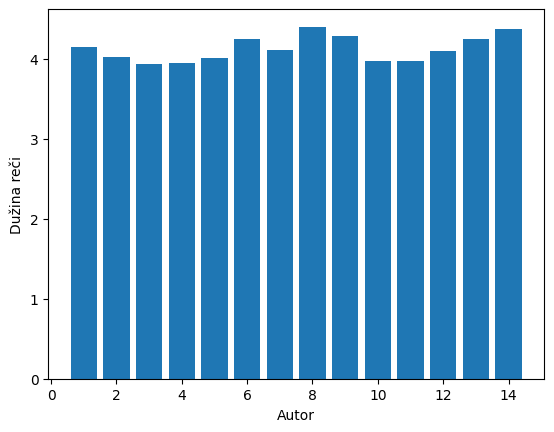
\includegraphics[width=\textwidth]{reci.png}
        \renewcommand{\thefigure}{} 
        \captionsetup{labelformat=empty}
        \subcaption{\textbf{Dužina reči po autorima.}}
        \label{fig:udeo1}
    \end{minipage}\hfill
    \begin{minipage}{0.4\textwidth}
        \centering
        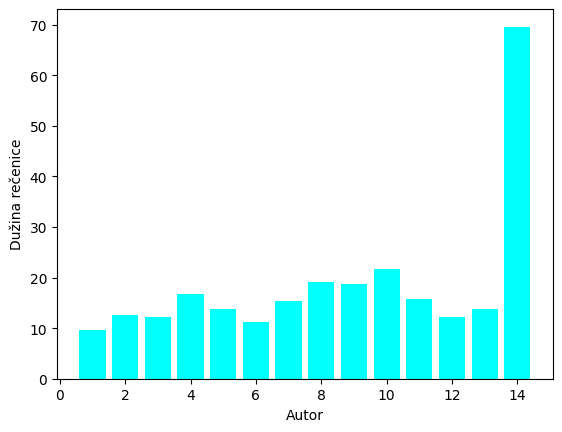
\includegraphics[width=\textwidth]{recenice.png}
        \renewcommand{\thefigure}{} 
        \captionsetup{labelformat=empty}
        \subcaption{\textbf{Dužina rečenica po autorima.}}
        \label{fig:udeo2}
    \end{minipage}
    \vskip\floatsep % dodatni vertikalni razmak između slika
    \begin{minipage}{0.4\textwidth}
        \centering
        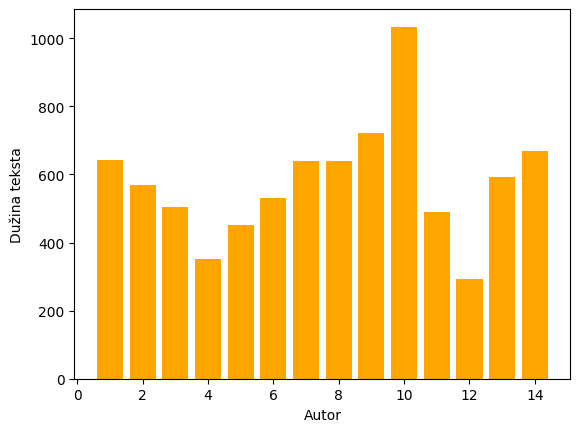
\includegraphics[width=\textwidth]{tekst.png}
        \renewcommand{\thefigure}{} 
        \captionsetup{labelformat=empty}
        \subcaption{\textbf{Dužina teksta po autorima.}}
        \label{fig:udeo3}
    \end{minipage}
\end{figure}



\newpage

\subsubsection{Formiranje modela} 
\begin{flushleft}
Nakon svega odrađenog, primenili smo dva različita modela za klasifikaciju.

\textbf{Random Forest} iz biblioteke sklearn je ansambl model, odnosno kombinacija više modela da bi se postigao bolji rezultat. Sastoji se od velikog broja stabala odlučivanja (decision trees), gde svako stablo uči na slučajnom podskupu podataka i daje svoju klasifikaciju. Konačna klasifikacija je rezultat glasanja svih stabala.\\
\textbf{Multinomial Bayes} iz biblioteke skelarn je probabilistički model zasnovan na Bajesovoj teoremi. Multinomijalni se odnosi na distribuciju verovatnoća koja se koristi za modeliranje više klasa.\\

Bajesova teorema je matematički izraz koji opisuje uslovnu verovatnoću događaja A, dajući određeni događaj B. Teorema se formuliše na sledeći način:
\begin{equation*}
P(A|B) = \frac{P(B|A) \cdot P(A)}{P(B)}
\end{equation*}
\end{flushleft} 
\subsubsection{Metrike, performanse modela} 
\begin{flushleft}
\textbf{Tačnost (accuracy):} \\
Tačnost meri koliko često model ispravno klasifikuje instance. Visoka tačnost ukazuje na dobar ukupan uspeh tj. performans modela.  Međutim, može biti obmanjujuća kada je jedna klasa značajno manje zastupljena od druge. Tada, model može postići visoku tačnost predviđajući dominantnu klasu, bez obzira na performanse na manje zastupljenoj klasi.\\
\[
\text{Tačnost} = \frac{\text{Broj tačno pozitivnih} + \text{Broj tačno negativnih}}{\text{Ukupan broj instanci}}
\]\vspace{1mm}


\textbf{Odziv (recall):}\\
Odziv, takođe poznat kao osetljivost (sensitivity) ili pravilnost (true positive rate), meri koliki je procenat stvarno pozitivnih instanci ispravno identifikovanih od strane modela. Odziv se često koristi kada je bitno minimizirati lažno negativne slučajeve.\\


\[
\text{Odziv} = \frac{\text{Broj tačno pozitivnih}}{\text{Broj tačno pozitivnih} + \text{Broj lažno negativnih}}
\]\vspace{1mm}

\textbf{F1-ocena (F1-score)}:\\
F1-ocena je harmonijska sredina između preciznosti i odziva. Ova mera pruža uravnotežen pogled na tačnost klasifikacije i uzima u obzir oba tipa grešaka (lažno pozitivne i lažno negativne). Visoka vrednost F1 ocene ukazuje na dobar balans između preciznosti i odziva.\\
\[
\text{F1 Score} = \frac{2 \cdot \text{Preciznost} \cdot \text{Odziv}}{\text{Preciznost} + \text{Odziv}}
\] 




%\vspace{1mm}

\begin{center}
\begin{table}[h]
\centering
\begin{tabular}{lccc}
\hline
\textbf{Model} & \textbf{Tačnost} & \textbf{F1 ocena} & \textbf{Odziv} \\
\hline
\textbf{Random Forest - Trening skup} & 0.6667 & 0.6468 & 0.6667 \\
\textbf{Random Forest - Test skup} & 0.2143 & 0.1827 & 0.2143 \\
\textbf{Multinomijalni Bajes - Trening skup} & 0.1667 & 0.1079 & 0.1667 \\
\textbf{Multinomijalni Bajes - Test skup} & 0.1429 & 0.0815 & 0.1429 \\
\hline
\end{tabular}
\caption*{Rezultati modela na trening i test skupovima}
\label{tab:rezultati}
\end{table}


\end{center}


\textbf{Analiza:\\}
Random Forest model pokazuje znatno bolje performanse na trening skupu u odnosu na test skup, što može ukazivati na prenaučenost/preprilagođavanje (overfitting).
Multinomijalni Bajes model takođe ima niske performanse, ali se generalno loše ponaša i na trening i na test skupu.
Random Forest model ima višu tačnost, F1 ocenu i odziv u poređenju sa Multinomial Bajes modelom na oba skupa podataka. U ovom konkretnom slučaju, Random Forest model ima bolje performanse u odnosu na Multinomijalnog Bajesa, čak i sa prenaučenošću na trening skupu.



\end{flushleft}


\newpage



\subsection{Set-fit i Sentence transformers biblioteke}

\begin{flushleft}
Prethodne metode nisu dale dobre rezultate, pa je istraživanje za dobrim algoritmima za analizu i klasifikaciju teksta postalo mnogo dublje i temeljnije. Zato smo odlučile primeniti biblioteke Set-fit i Sentence transformers.
    \vspace{2mm}

Program koji vrši ove operacije se nalazi u set\textunderscore fit.ipynb 
datoteci.\\ \vspace{2mm}

Prvo, uvoze se neophodnosti za rad: biblioteka pandas, klase SetFitModel i 
SetFitTrainer iz setfit biblioteke, Datasets iz datasets biblioteke, funkcije 
load\textunderscore datasets iz datasets biblioteke i train\textunderscore 
test\textunderscore split iz biblioteke sklearn.\\ \vspace{2mm}


Set-fit je okvir za fina podešavanja Sentence Transformer modela sa malim brojem primera za učenje. Generalno postiže visoku tačnost sa malo označenih podataka. \\ \vspace{2mm}

Klasa Datasets sadrži funkcionalnosti za rad s različitim skupovima podataka, omogućujući upravljanje i pristup različitim skupovima podataka. Funkcija load\textunderscore datasets može biti korisna za učitavanje specifičnog skupa podataka u program. \\ \vspace{2mm}

Opet, izbacujemo kolone koje nam neće uticati na rezultate. Dodaje se nova kolona \texttt{"label"} koja se generiše konvertovanjem kolone \texttt{"Autor"} u numerički kod preko odredjenih metoda. Metoda astype('category') se koristi za promenu tipa podataka kolone u 'category', a kada se kolona tretira kao kategorička, mogu se koristiti kategoričke operacije, uključujući i dodeljivanje numeričkih kodova kategorijama. Metoda cat.codes se primenjuje na kategoričku seriju i dodeljuje numeričke kodove svakoj kategoriji tako da svaka jedinstvena vrednost u koloni \texttt{"Autor"} dobija svoj jedinstveni numerički kod. Zatim se uklanja originalna kolona \texttt{"Autor"} i menja naziv kolone \texttt{"Tekst"} u \texttt{"text"}. Pretvaranje u numeričke podatke je neophodno kod korišćenja ove biblioteke. Trenutne promene na bazi su sačuvane u setfit\textunderscore medjukorak.csv datoteci. Podaci se dalje pretvaraju u Dataset objekat, a zatim se vrši podela podataka na trening i test skupove u odnosu 80:20. \\Inicijalizuje se model za procenu sličnosti rečenica, koristeći prethodno treniran model \texttt{sentence-transformers/paraphrase-multilingual-mpnet-base-v2}. Definiše se funkcija make\textunderscore model, koja pravi novi model na osnovu prethodno treniranog modela. On je treniran tako da grupiše rečenice po semantičkoj sličnosti koji u pozadini koristi logističku regresiju. Zatim se inicijalizuje trener sa određenim parametrima, uključujući model, trening i evaluacione skupove, funkciju gubitka (loss function), veličinu podskupa (batch size) i druge relevantne parametre. Definiše se funkcija hyperparameter\textunderscore search\textunderscore function koja se koristi za pretragu hiperparametara tokom treninga. Međutim, zbog jako dugog treniranja samog modela bez pretraživanja hiperparametra, odustali smo od korišćenja ove funkcije, jer dosta prolonigra vreme izvršavanja. Vrši se trening modela na trenutno postavljenim parametrima i evaluacija treniranog
modela. Kada se koristi set fit klasifikacija, često je bitnije da se očuva redosled i odnosi između klasa, a ne apsolutne vrednosti numeričkih kodova. Algoritmi poput SetFit-a koriste reprezentaciju podataka koja je rezultat prethodno treniranog modela (Sentence Transformer) i ne zavise direktno od numeričkih vrednosti ciljne promenljive.


\vspace{2mm}
\subsubsection{Metrike, performanse modela} 

\begin{center}
  \begin{table}[h]
    \centering
    \begin{tabular}{lccc}
      \hline
      & \textbf{Tačnost} \\
      \hline
      \textbf{Trening skup} & 1.0 \\
     \textbf{ Test skup} & 0.2857 \\
      \hline
    \end{tabular}
    \caption*{Rezultati SetFit modela na trening i test skupovima}
    \label{tab:setfit_results}
  \end{table}
\end{center}

\textbf{Analiza:}\\
Dolazi do preprilagođavanja. To se može zaključiti iz toga što je tačnost na trening skupu 100\%. Ovakva situacija je dovela do prilagođavanja trening podacima što prouzrokuje lošu klasifikaciju na novim, test podacima.


\end{flushleft}

\newpage


\subsection{Rekurentne neuronske mreže}

\begin{flushleft}

Uvezene su sve potrebne biblioteke, slojevi, funkcije i optimizatori. To su pandas
biblioteka, "tensorflow" bliblioteka a iz nje: slojevi Embedding, LSTM i Dense, 
funkcija pad\textunderscore sequences, klasa Sequential, funkcija EarlyStoping i
Adam optimizator.\\
Izbrisane nepotrebne kolone, sva velika slova pretvorena u mala, podaci podeljeni 
na trening i test skupove.    \\
\vspace{4pt}

Program koji vrši ove operacije se nalazi u rnn.ipynb datoteci.\\ \vspace{1.5mm}

Korišćena je EarlyStopping, tehnika za automatsko zaustavljanje treninga neuronske 
mreže, kada određeni metrički pokazatelji prestanu poboljšavati na validacionom 
skupu tokom treninga. Ovo pomaže u sprečavanju preprilagodjavanja (overfittinga) i
omogućava modelu da prestane sa treniranjem čim prestane poboljšanje performansi.\\


U ovom konkretnom slučaju:\\

\hspace{40pt}- patience = 3: Predstavlja broj epoha bez poboljšanja pre nego što 
trening bude\\ \hspace{44pt} zaustavljen,   u ovom slučaju, trening će biti 
zaustavljen nakon tri uzastopne epohe bez \\ \hspace{47pt}napretka.\\

\hspace{40pt}- monitor = 'val\textunderscore accuracy': Ova opcija definiše metriku 
koja će biti praćena kako bi se \\ \hspace{47pt}odlučilo da li je došlo do 
poboljšanja. U ovom slučaju, prati se tačnost na validacionom \\ 
\hspace{47pt}skupu.\\

\hspace{40pt}- restore\textunderscore best\textunderscore weights=True: Ova opcija 
omogućava automatsko vraćanje težina modela sa \\ \hspace{46pt}epohe u kojoj je 
postignuta najbolja tačnost na validacionom skupu. To znači da će model \\ 
\hspace{46pt}biti sačuvan u trenutku kada je validaciona tačnost bila najbolja.\\

\vspace{4pt}
Tekstualni podaci su pretvoreni u sekvence, a zatim su postavljene sekvence na
fiksan broj koristeći pad\textunderscore sequences.\\



Korišćen je model sa ugnježdenim slojem (Embedding layer), LSTM slojem, i gusto 
povezanim slojem sa softmax aktivacijom kako bi se vršila klasifikacija autora.\\
Kompajliran je model koristeći kategoričku entropiju kao funkciju gubitka i Adam 
optimizator.\\

Model je treniran na trening podacima sa definisanim brojem epoha i ranim 
zaustavljanjem u slučaju da nema poboljšanja na validacionom skupu.\\

Na kraju, model je evaluiran na test podacima, a rezultati su dobijeni korišćenjem
model.evaluate i model.predict.\\


\vspace{2mm}
\subsubsection{Metrike, performanse modela} 

\begin{center}
  \begin{table}[h]
    \centering
    \begin{tabular}{lccc}
      \hline
      & \textbf{Tačnost} \\
      \hline
      \textbf{Trening skup} & 0.35 \\
      \textbf{Test skup} & 0.18 \\
      \hline
    \end{tabular}
    \caption*{Rezultati rekurentnih neuronskih mreža na trening i test skupovima}
    \label{tab:setfit_results}
  \end{table}
\end{center}

\textbf{Analiza:}\\
Model je generalno jako loš. Tačnost na trening podacima da bude 24\% je jako loše. Ta loša prilagodjenost na trening skupu, dovodi do neutreniranog modela koji ne ume da se snađe sa nepoznatim i novim podacima.


\end{flushleft}

\newpage




\subsection{Classla biblioteka}

\begin{flushleft}

Classla omogućava obradu standardnog slovenačkog, hrvatskog, srpskog i bugarskog jezika na nivoima tokenizacije i razdvajanja rečenica, označavanja vrste reči, lematizacije
analize zavisnosti itd. Na kraju, omogućava obradu nestandardnog (internet) slovenačkog, hrvatskog i srpskog jezika na istim nivoima kao i standardni jezik (svi modeli su prilagođeni nestandardnom jeziku, osim za analizu zavisnosti gde se koristi standardni modul).  \\    \vspace{2mm}


Uvozi se biblioteka Classla, klasa FreqDist (koristi se za praćenje broja pojavljivanja različitih elemenata u korpusu teksta) iz nltk biblioteke i skidaju se potrebni resursi za srpski jezik.\\    \vspace{2mm}

Program koji vrši ove operacije se nalazi u classla.ipynb datoteci.\\ \vspace{1.5mm}

   Napravi se pipeline (niz procesa/koraka) za obradu teksta na srpskom jeziku koji
   uključuje tri procesora: tokenize, lemma, i pos.\\
  \hspace*{25pt}- Tokenize - Ovaj korak se bavi razbijanjem teksta na pojedinačne reči ili tokene. \\
   \hspace*{25pt}- Lemma - Lematizacija se koristi za određivanje osnovnih oblika 
   reči. Na primer, \\ \hspace*
   {27pt} lematizacija za reč \texttt{"trče"} je vraća u osnovni 
   oblik tj. "trčati". Ovo omogućava da se iste reči\\ \hspace*
   {27pt} u drugačijem obliku posmatraju kao iste.\\
   \hspace*{25pt}- POS (Part-of-Speech): Ovaj korak se bavi određivanjem vrste reči 
   (npr. imenica, glagol, \\ \hspace*
   {31pt}pridev) za svaki token u tekstu. To je 
   korisno za razumevanje gramatičke strukture rečenice.\\
   \vspace{2pt}

    Tekst se procesuira kroz definisani Classla pipeline, i dobija se objekat doc.
    Iz njega se izdvajaju leme (osnovni oblici reči) za svaku reč u tekstu. Leme 
    se dodaju u listu lemmas.\\

Funkcija process\textunderscore text se primenjuje na svaki red u koloni \texttt{"Tekst"}. Rezultat, odnosno lista lema, se dodaje u novu kolonu \texttt{"Procesiran tekst"}. Opet je definisana funkcija remove\textunderscore  punctuation  kao i u stilometrijskoj analizi. Definiše se funkcija remove\textunderscore freq\textunderscore words u kojoj se: računa frekvencija reči i najfrekventnijih 100 reči se izdvoji zajedno sa njihovim 
brojem pojavljivanja. Zatim se reči koje imaju broj pojavljivanja veći od 100 ili 
su veoma kratke (1 ili 2) uklanjaju. Ova funkcija se dalje primeni na svaki red u 
koloni \texttt{"Procesiran tekst"}. Ova funkcija može biti korisna radi izostavljanja reči koje su veoma česte i ne nose puno semantičkog značenja u analizi teksta. Ovo može pomoći u fokusiranju na reči koje su potencijalno relevantne ili značajne za analizu. Trenutne promene na bazi su sačuvane u classla\textunderscore medjukorak.csv datoteci.
\vspace{2pt}
Dalje, uvozimo klasu TfidfVectorizer iz biblioteke sklearn. 
Prvo se za svakog autora spajaju tekstovi pesama u jedan tekst pojedinačno.
Koristi se TfidfVectorizer za izračunavanje TF-IDF vrednosti (mera koja ima za cilj
izdvojiti reči koje su značajne za jedan dokument u odnosu na ostatak dokumenata). 
Parametar max\textunderscore features=3000 ograničava broj reči koje će biti uzete 
u obzir na osnovu njihove frekvencije. Trenutne promene na bazi su sačuvane u classla\textunderscore tfidf.csv datoteci.
\hspace{3pt} \[ \text{TF}(t, d) = \frac{\text{broj pojavljivanja reči } t \text{ u
dokumentu } d}{\text{ukupan broj reči u dokumentu } d} \]
\hspace{3pt} \[ \text{IDF}(t, D) = \log\left(\frac{\text{ukupan broj dokumenata u 
korpusu } D}{\text{broj dokumenata koji sadrže reč } t + 1}\right) \]
\hspace{3pt} \[ \text{TF-IDF}(t, d, D) = \text{TF}(t, d) \times \text{IDF}(t, D) 
\] \\
\vspace{3pt}
\hspace{60pt}t - reč koja se analizira u trenutnom kontekstu;\\
\hspace{60pt}d - trenutni dokument u kojem se meri frekvencija reči;\\
\hspace{60pt}D - ceo korpus dokumenata u kom se meri frekvencija reči u odnosu na 
sve dokumente;
\vspace{4pt}

\vspace{7pt}
Sledeća je podela na trening i test skupove u odnosu 80:20 uz stratifikaciju po koloni \verb|"Autor"|.
\end{flushleft}


\newpage




\subsubsection{Metrike koje ćemo koristiti}



%%%%%%%%%%%%%%%%%%%%%
\begin{flushleft}
    
\textbf{Makro-preciznost (Macro-Precision):}\\
Makro-preciznost se računa kao prosečna preciznost za svaku klasu. Preciznost za svaku klasu se računa kao broj tačno pozitivnih instanci te klase podeljen sa zbirom tačno pozitivnih i lažno pozitivnih instanci za tu klasu. Makro-preciznost je zatim prosečna vrednost ovih preciznosti za sve klase.\\
\[
\text{Makro-preciznost} = \frac{1}{N} \sum_{i=1}^{N} \frac{\text{TP}_i}{\text{TP}_i + \text{FP}_i}
\]
\vspace{2.75mm}

\textbf{Makro-odziv (Macro-Recall):}\\
Makro-odziv se računa kao prosečan odziv (takođe poznat kao osetljivost ili pravilnost) za svaku klasu. Odziv za svaku klasu se računa kao broj tačno pozitivnih instanci te klase podeljen sa zbirom tačno pozitivnih i lažno negativnih instanci za tu klasu. Makro-odziv je zatim prosečna vrednost ovih odziva za sve klase. \\
\[
\text{Makro-odziv} = \frac{1}{N} \sum_{i=1}^{N} \frac{\text{TP}_i}{\text{TP}_i + \text{FN}_i}
\]
\vspace{2.75mm}

\textbf{Makro F1-ocena (Macro F1-Score):}\\
Makro F1 ocena predstavlja srednju vrednost F1 ocena za svaku klasu (definicija F1 ocene objašnjena u 3.1.3 poglavlju).\\
\[
\text{Makro F1} = \frac{1}{N} \sum_{i=1}^{N} F1_i
\]

\vspace{2.75mm}
\textbf{Makro podrška (Macro Support):}\\
Makro podrška predstavlja ukupan broj instanci u svim klasama, bez obzira na neravnotežu između klasa. To znači da svaka klasa doprinosi jednako u izračunavanju makro prosečnih vrednosti. 

\[
\text{Macro Podrška} = \sum_{i=1}^{C} \text{Podrška}_i
\]
\vspace{2.75mm}


\textbf{Težinska prosečna preciznost (Weighted Average Precision):}\\
Weighted Average Precision u kontekstu klasifikacionih modela označava prosečnu vrednost preciznosti uzetu sa težinama u obziru. Preciznost meri tačnost pozitivnih predikcija za određenu klasu, a težinska prosečna preciznost se koristi kada imamo nebalansirane klase.  \\


\[
\text{Težinska prosečna preciznost} = \frac{\sum_{i=1}^{C} (\text{Preciznost}_i \times \text{Podrška}_i)}{\text{Ukupna podrška}}
\]
\hspace{5cm} gde je C ukupan broj klasa.
\vspace{2.75mm}


\textbf{Težinski prosečni odziv (Weighted Average Recall): }\\
Težinski prosečan odziv je metrika koja se koristi kako bi se uzela u obzir neravnoteža između klasa prilikom računanja prosečnog odziva. \\
\[
\text{Težinski prosečni odziv} = \frac{\sum_{i=1}^{C} (\text{Odziv}_i \times \text{Podrška}_i)}{\text{Ukupna podrška}}
\]
\vspace{2.75mm}

\newpage

\textbf{Težinska prosečna F1-ocena (Weighted average F1-score):}\\
Težinska prosečna F1-ocena predstavlja srednju vrednost F1-skorova za svaku klasu, pri čemu se uzimaju u obzir težine kako bi se uračunala neravnoteža između klasa u skupu podataka. 

\[
\text{Težinska prosečna F1-ocena} = \frac{\sum_{i=1}^{C} (\text{F1 ocena}_i \times \text{Podrška}_i)}{\text{Ukupna podrška}}
\]

\vspace{2.75mm}

\textbf{Težinska prosečna podrška (Wighted Average Support):}\\
Makro podrška predstavlja ukupan broj instanci u svim klasama, bez obzira na neravnotežu između klasa. To znači da svaka klasa doprinosi jednako u izračunavanju makro prosečnih vrednosti. 


\[
\text{Težinska proesčna podrška} = \frac{\sum_{i=1}^{C} (\text{Podrška}_i \times \text{Težina}_i)}{\sum_{i=1}^{C} \text{Težina}_i}
\]
\vspace{2.75mm}

\textbf{Matrica konfuzuije (confusion matrix):} \\
Matrica konfuzije je tabela koja se koristi u problemima klasifikacije kako bi se prikazala performansa modela na testiranju. Ova matrica upoređuje stvarne vrednosti ciljne promenljive sa predviđenim vrednostima od strane modela. Evo kako je matrica konfuzije obično organizovana: \\
\[
\begin{bmatrix}
\text{Stvarno negativno (TN)} & \text{Lažno pozitivno (FP)} \\
\text{Lažno negativno (FN)} & \text{Stvarno pozitivno (TP)}
\end{bmatrix}
\]
\begin{center}
(TN): Broj instanci koje su ispravno klasifikovane kao negativne;\\
(FP): Broj instanci koje su pogrešno klasifikovane kao pozitivne;\\
(FN): Broj instanci koje su pogrešno klasifikovane kao negativne;\\
(TP): Broj instanci koje su ispravno klasifikovane kao pozitivne;\\
    
\end{center}


\vspace{2.75mm}

\textbf{ROC kriva (ROC curve):}\\
ROC kriva je grafički prikaz performansi klasifikacionog modela koja ilustruje sposobnost modela da razlikuje pozitivne i negativne instance (klase). ROC kriva se generiše variranjem praga odlučivanja (eng. decision threshold) klasifikacionog modela. Prag odlučivanja je vrednost koja se koristi da se odredi kojoj klasi pripada instanca na osnovu izlaza modela. Na x-osi ROC krive se obično nalazi stopa lažno pozitivnih, koja predstavlja udeo negativnih instanci koje su netačno klasifikovane kao pozitivne. Na y-osi se nalazi Stopa istinito pozitivnih, koja predstavlja udeo pozitivnih instanci koje su tačno klasifikovane kao pozitivne. Idealna ROC kriva biće pravac koji ide od donjeg levog ugla do gornjeg desnog ugla grafa, što znači da model ima visoku sposobnost razlikovanja između klasa bez obzira na prag odlučivanja.
\vspace{2.75mm}

\textbf{AUC - površina ispod ROC krive (Area Under Curve):} \\
AUC je mera koja kvantifikuje celokupnu performansu modela. Što je AUC bliže 1, to znači da je model bolji u razlikovanju između klasa. 
\vspace{2.75mm}

Objašnjenje za tačnost i F1-ocenu možemo videti na strani 5.


\end{flushleft}


%%%%%%%%%%%%%%%%%%


\subsubsection{Klasifikacioni algoritmi koje ćemo koristiti za treniranje modela}
\begin{flushleft}

Za algoritme Random Forest i Multinomial Bayes, objašnjenje možemo videti na strani 5.
\vspace{2.75mm}


\textbf{Gradient Boosting:}\\
Gradient Boosting je ansambl algoritam koji gradi niz slabih modela, obično drvo odlučivanja, gde svaki novi model ispravlja greške prethodnih. Modeli se dodaju postepeno, uz težine prilagođene greškama prethodnih modela.
\vspace{2.75mm}

\textbf{Support Vector Classifier (SVC):}\\
SVC je algoritam za klasifikaciju koji gradi hiper-ravan za razdvajanje različitih klasa. Cilj je pronaći ravan koja maksimizuje marginu između klasa.



\end{flushleft}


\newpage
\subsubsection{Klasifikacioni modeli i njihovi rezultati}
\begin{flushleft}
\vspace{1mm}

U nastavku ćemo pominjati GridSearch, što predstavlja tehniku optimizacije hiperparametara koja se često koristi u mašinskom učenju kako bi se pronašle optimalne vrednosti hiperparametara za neki model. Hiperparametri su parametri koji nisu naučeni tokom treninga modela, već se moraju postaviti pre treniranja. 
GridSearch radi tako što definiše skup vrednosti za svaki hiperparametar koji želimo optimizovati, a zatim sistematski prolazi kroz sve kombinacije ovih vrednosti. Za svaku kombinaciju hiperparametara, trenira se model koristeći određene vrednosti i ocenjuje se pomoću unapred definisane metrike performansi, kao što je tačnost, preciznost, ili neka druga relevantna metrika.

\end{flushleft}

\vspace{2.5mm}
\paragraph{Gradient Boosting}
\begin{flushleft}
Napravljen je model sa najboljim vrednostima hiperparametara  dobijenih primenom GridSearch-a. \\
\texttt{GradientBoostingClassifier(learning\textunderscore rate=0.1, 
max\textunderscore depth=3, min\textunderscore samples\textunderscore split=5, 
min\textunderscore samples\textunderscore leaf=4, n\textunderscore estimators=100)}


\begin{itemize}
\item \textbf{Klasifikacioni izveštaj (classification report):}
\end{itemize}

\begin{table}[ht]
    \centering*
    \begin{tabular}{cccccc}
        \textbf{Klasa} & \textbf{Preciznost} & \textbf{Odziv} & \textbf{F1-ocena} & \textbf{Podrška} \\
        \hline
        1 & 0.00 & 0.00 & 0.00 & 1 \\
        2 & 0.25 & 0.50 & 0.33 & 2 \\
        3 & 1.00 & 0.50 & 0.67 & 2 \\
        4 & 0.12 & 0.50 & 0.20 & 2 \\
        5 & 0.33 & 0.50 & 0.40 & 2 \\
        6 & 1.00 & 0.50 & 0.67 & 2 \\
        7 & 0.00 & 0.00 & 0.00 & 1 \\
        8 & 0.00 & 0.00 & 0.00 & 3 \\
        9 & 1.00 & 0.50 & 0.67 & 2 \\
        10 & 1.00 & 0.50 & 0.67 & 2 \\
        11 & 0.50 & 0.50 & 0.50 & 2 \\
        12 & 0.00 & 0.00 & 0.00 & 2 \\
        13 & 0.00 & 0.00 & 0.00 & 3 \\
        14 & 0.00 & 0.00 & 0.00 & 2 \\
        \hline
        \textbf{Macro Avg} & 0.37 & 0.29 & 0.29 & 28 \\
        \textbf{Weighted Avg} & 0.37 & 0.29 & 0.29 & 28 \\
    \end{tabular}

    \label{tab:classification-report}
\end{table}

\begin{itemize}
\item \textbf{Tačnost Gradient Boosting modela: 0.29}
\item \textbf{F1-ocena Gradient Boosting modela: 0.29}
\end{itemize}


\vspace{3mm}
U nastavku možemo videti matricu konfuzije i ROC krivu zajedno sa AUC vrednosti za Gradient Boosting algoritam.
\end{flushleft}

\newpage


\begin{figure}[ht]
    \begin{minipage}{0.5\textwidth}
        \centering
        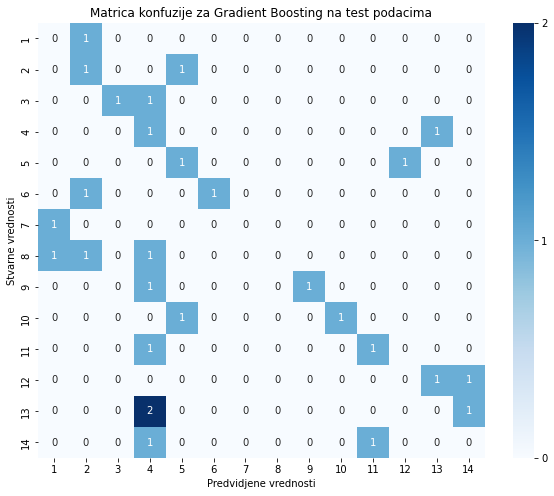
\includegraphics[width=\linewidth]{gradientconf.png}
        \captionsetup{justification=centering}
        \caption*{\textbf{Matrica konfuzije za Gradient \\Boosting model.}}
        \label{fig:nedostajuce}
    \end{minipage}%
    \begin{minipage}{0.5\textwidth}
        \textbf{Analiza:}\\
        
        \vspace{1mm}
        Element na poziciji (2, 2): 1\\
        Element na poziciji (3, 3): 1\\
        Element na poziciji (4, 4): 1\\
        Element na poziciji (5, 5): 1\\
        Element na poziciji (6, 6): 1\\
        Element na poziciji (9, 9): 1\\
        Element na poziciji (10, 10): 1\\
        Element na poziciji (11, 11): 1\\
    \end{minipage}
\end{figure}
\begin{flushleft}

Gledamo sve nenula elemente na dijagonali matrice konfuzije. Što ih je više, to znači da postoje instance koje su tačno klasifikovane u određenu klasu. Ovi elementi označavaju situacije gde su modeli tačno klasifikovali instance za određene klase. Klase 2, 3, 4, 5, 6, 9, 10 i 11 su dobro klasifikovane. 

\end{flushleft}

%\newpage
\begin{flushleft}
 

\begin{figure}[ht]
    \centering
    \begin{minipage}{0.5\textwidth}
        \centering
        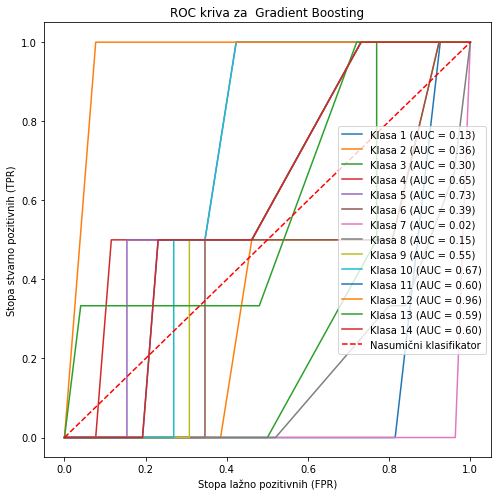
\includegraphics[width=\textwidth]{gradientROC.png}
        \renewcommand{\thefigure}{} 
        \captionsetup{labelformat=empty}
        \subcaption{\textbf{ROC krive svih klasa.}}
        \label{fig:udeo1}
    \end{minipage}\hfill
    \begin{minipage}{0.5\textwidth}
        \centering
        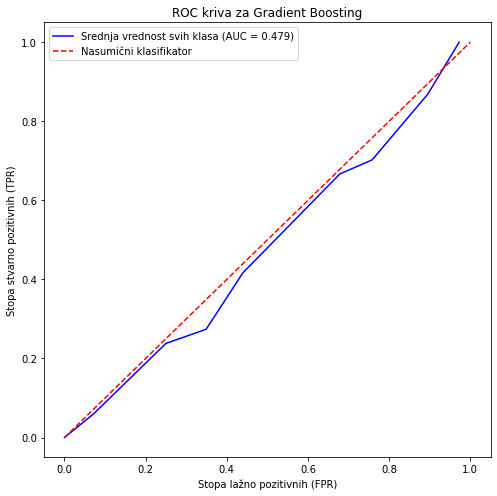
\includegraphics[width=\textwidth]{prosecniROC/gradient.png}
        \renewcommand{\thefigure}{} 
        \captionsetup{labelformat=empty}
        \subcaption{\textbf{ROC kriva - prosek svih klasa.}}
        \label{fig:udeo2}
    \end{minipage}
\end{figure}


Po AUC vrednostima i samom položaju krivih u odnosu na nasumični klasifikator (prava y=x), možemo videti da je klasa 12 najbolje klasifikovana, a klasa 7 najgore. Slika b pokazuje ROC krivu proseka svih klasa na kojoj možemo videti da je klasifikator malo ispod nasumičnog klasifikatora koji prikazuje granicu izmedju lošeg i dobrog klasterovanja. To znaci da je ovaj algoritam malo gori od "proseka".

    
\end{flushleft}
\newpage
\vspace{2mm}
\paragraph{Random Forest}
\begin{flushleft}
Napravljen je model sa najboljim vrednostima hiperparametara  dobijenih primenom GridSearch-a.
\texttt{RandomForestClassifier(max\textunderscore depth=5,min\textunderscore 
samples\textunderscore split=15, n\textunderscore estimators=300)}    
\end{flushleft}

\begin{itemize}
    \item \textbf{Klasifikacioni izveštaj (classification report):}
\end{itemize}

\begin{table}[ht]
    \centering
    \begin{tabular}{cccccc}
        \textbf{Klasa} & \textbf{Preciznost} & \textbf{Odziv} & \textbf{F1-ocena} & \textbf{Podrška} \\
        \hline
        1 & 0.00 & 0.00 & 0.00 & 1 \\
        2 & 0.00 & 0.00 & 0.00 & 2 \\
        3 & 1.00 & 0.50 & 0.67 & 2 \\
        4 & 0.17 & 0.50 & 0.25 & 2 \\
        5 & 0.20 & 0.50 & 0.29 & 2 \\
        6 & 0.00 & 0.00 & 0.00 & 2 \\
        7 & 0.00 & 0.00 & 0.00 & 1 \\
        8 & 0.38 & 1.00 & 0.55 & 3 \\
        9 & 0.00 & 0.00 & 0.00 & 2 \\
        10 & 0.00 & 0.00 & 0.00 & 2 \\
        11 & 0.00 & 0.00 & 0.00 & 2 \\
        12 & 0.00 & 0.00 & 0.00 & 2 \\
        13 & 0.12 & 0.33 & 0.18 & 3 \\
        14 & 0.00 & 0.00 & 0.00 & 2 \\
        \hline
        \textbf{Macro Avg} & 0.13 & 0.20 & 0.14 & 28 \\
        \textbf{Weighted Avg} & 0.15 & 0.25 & 0.16 & 28 \\
    \end{tabular}
    \label{tab:classification-report-random-forest}
\end{table}

\begin{itemize}
    \item \textbf{Tačnost Random Forest modela:} 0.25
    \item \textbf{F1-ocena Random Forest modela:} 0.16
\end{itemize}


\begin{figure}[ht]
    \begin{minipage}{0.5\textwidth}
        \centering
        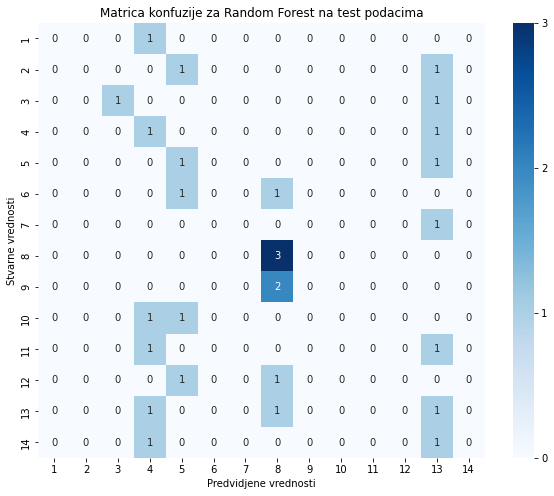
\includegraphics[width=\linewidth]{forestconf.png}
        \captionsetup{justification=centering}
        \caption*{\textbf{Matrica konfuzije za Random \\Forest model.}}
        \label{fig:nedostajuce}
    \end{minipage}%
    \begin{minipage}{0.5\textwidth}
        \textbf{Analiza:}\\
        
        \vspace{1mm}
        Element na poziciji (3, 3): 1\\
        Element na poziciji (4, 4): 1\\
        Element na poziciji (5, 5): 1\\
        Element na poziciji (8, 8): 3\\
        Element na poziciji (9, 9): 1\\
        Element na poziciji (13, 13): 1\\
    \end{minipage}
\end{figure}
\begin{flushleft}

Klase 3, 4, 5, 8 i 13 su dobro klasifikovane. Model je tačno klasifikovao čak 3 instance za klasu 8.

\end{flushleft}
\newpage



\begin{figure}[ht]
    \centering
    \begin{minipage}{0.5\textwidth}
        \centering
        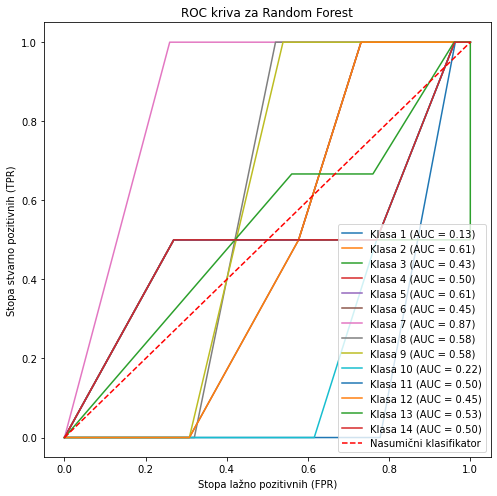
\includegraphics[width=\textwidth]{forestROC.png}
        \renewcommand{\thefigure}{} 
        \captionsetup{labelformat=empty}
        \subcaption{\textbf{ROC krive svih klasa.}}
        \label{fig:udeo1}
    \end{minipage}\hfill
    \begin{minipage}{0.5\textwidth}
        \centering
        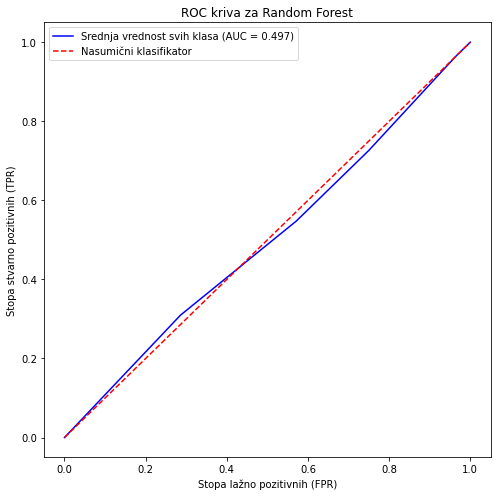
\includegraphics[width=\textwidth]{prosecniROC/forest.png}
        \renewcommand{\thefigure}{} 
        \captionsetup{labelformat=empty}
        \subcaption{\textbf{ROC kriva - prosek svih klasa.}}
        \label{fig:udeo2}
    \end{minipage}
\end{figure}
\begin{flushleft}

Možemo videti da je klasa 7 najbolje klasifikovana, a klasa 1 najgore. Slika b pokazuje ROC krivu proseka svih klasa na kojoj možemo videti da je klasifikator malo ispod, a malo iznad nasumičnog klasifikatora koji prikazuje granicu izmedju lošeg i dobrog klasterovanja. To znaci da je ovaj algoritam prosečan u klasifikaciji.

\end{flushleft}

%\newpage
\vspace{3mm}

\paragraph{Multinomial Bayes}
\begin{flushleft}
Napravljen je model bez argumenata. \\


\begin{itemize}
\item \textbf{Klasifikacioni izveštaj (classification report):}
\end{itemize}
\begin{table}[ht]
    \centering
    \begin{tabular}{cccccc}
        \textbf{Klasa} & \textbf{Preciznost} & \textbf{Odziv} & \textbf{F1-ocena} & \textbf{Podrška} \\
        \hline
        1 & 0.00 & 0.00 & 0.00 & 1 \\
        2 & 0.00 & 0.00 & 0.00 & 2 \\
        3 & 0.00 & 0.00 & 0.00 & 2 \\
        4 & 1.00 & 0.50 & 0.67 & 2 \\
        5 & 0.00 & 0.00 & 0.00 & 2 \\
        6 & 0.00 & 0.00 & 0.00 & 2 \\
        7 & 0.00 & 0.00 & 0.00 & 1 \\
        8 & 0.43 & 1.00 & 0.60 & 3 \\
        9 & 0.00 & 0.00 & 0.00 & 2 \\
        10 & 0.00 & 0.00 & 0.00 & 2 \\
        11 & 0.00 & 0.00 & 0.00 & 2 \\
        12 & 0.00 & 0.00 & 0.00 & 2 \\
        13 & 0.17 & 1.00 & 0.29 & 3 \\
        14 & 0.00 & 0.00 & 0.00 & 2 \\
        \hline
        \textbf{Macro Avg} & 0.04 & 0.14 & 0.06 & 28 \\
        \textbf{Weighted Avg} & 0.06 & 0.21 & 0.09 & 28 \\
    \end{tabular}
    \label{tab:classification-report-multinomial-bayes}
\end{table}

\begin{itemize}
  \item \textbf{Tačnost za Mulitnomial Bayes model:} 0.21
    \item \textbf{F1-ocena za Multinomial Bayes model:} 0.09
\end{itemize}
\end{flushleft}


\begin{figure}[ht]
    \begin{minipage}{0.5\textwidth}
        \centering
        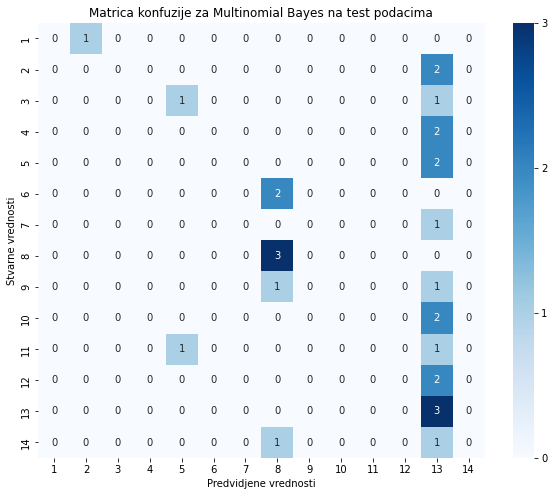
\includegraphics[width=\linewidth]{MBconf.png}
        \captionsetup{justification=centering}
        \caption*{\textbf{Matrica konfuzije za Multinomial \\Bayes model.}}
        \label{fig:nedostajuce}
    \end{minipage}%
    \begin{minipage}{0.5\textwidth}
        \textbf{Analiza:}\\
        
        \vspace{1mm}
        Element na poziciji (8, 8): 3\\
        Element na poziciji (13, 13): 3\\
    \end{minipage}
\end{figure}
\begin{flushleft}

Klase 8 i 13 su dobro klasifikovane. Model je tačno klasifikovao po 3 instance za te klase, ali nije pravilno klasifikovao ni jednu drugu klasu, što nije dobro.


%\newpage

\begin{figure}[ht]
    \centering
    \begin{minipage}{0.5\textwidth}
        \centering
        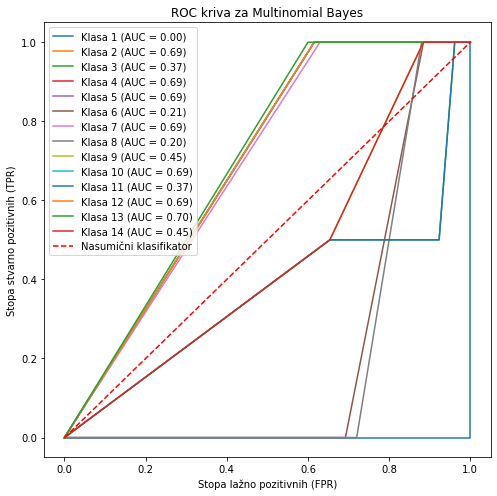
\includegraphics[width=\textwidth]{MbROC.png}
        \renewcommand{\thefigure}{} 
        \captionsetup{labelformat=empty}
        \subcaption{\textbf{ROC krive svih klasa.}}
        \label{fig:udeo1}
    \end{minipage}\hfill
    \begin{minipage}{0.5\textwidth}
        \centering
        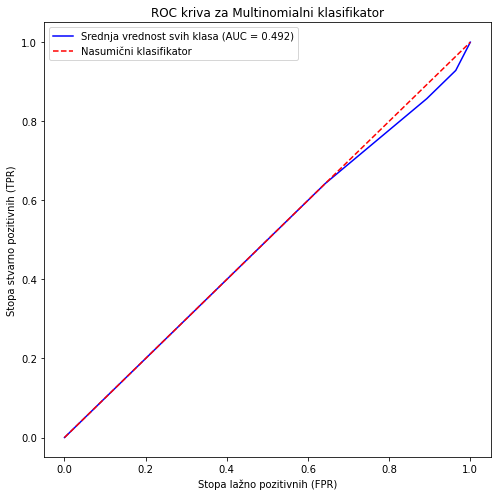
\includegraphics[width=\textwidth]{prosecniROC/multinomijalni.png}
        \renewcommand{\thefigure}{} 
        \captionsetup{labelformat=empty}
        \subcaption{\textbf{ROC kriva - prosek svih klasa.}}
        \label{fig:udeo2}
    \end{minipage}
\end{figure}


Možemo videti da su klase 2, 4, 5, 7, 10 i 12  najbolje klasifikovane, a klasa 1 najgore. Slika b pokazuje ROC krivu proseka svih klasa na kojoj možemo videti da je klasifikator malo iznad, a malo se preklapa sa nasumičnim klasifikatorom koji prikazuje granicu izmedju lošeg i dobrog klasterovanja. To znači da je ovaj algoritam prosečan u klasifikaciji.
\end{flushleft}


\newpage



\paragraph{SVC} 
\begin{flushleft}

Napravljen je model sa najboljim vrednostima hiperparametara  dobijenih primenom GridSearch-a. \\
\texttt{SVC(kernel='sigmoid', C=10, coef0=1.0, gamma='scale')}

\begin{itemize}
\item \textbf{Klasifikacioni izveštaj (classification report):}
\end{itemize}

\begin{table}[ht]
    \centering
    \begin{tabular}{cccccc}
        \textbf{Class} & \textbf{Precision} & \textbf{Recall} & \textbf{F1-Score} & \textbf{Support} \\
        \hline
        1 & 0.00 & 0.00 & 0.00 & 1 \\
        2 & 0.50 & 0.50 & 0.50 & 2 \\
        3 & 1.00 & 0.50 & 0.67 & 2 \\
        4 & 0.33 & 1.00 & 0.50 & 2 \\
        5 & 0.50 & 0.50 & 0.50 & 2 \\
        6 & 1.00 & 1.00 & 1.00 & 2 \\
        7 & 0.00 & 0.00 & 0.00 & 1 \\
        8 & 0.75 & 1.00 & 0.86 & 3 \\
        9 & 0.00 & 0.00 & 0.00 & 2 \\
        10 & 1.00 & 0.50 & 0.67 & 2 \\
        11 & 1.00 & 0.50 & 0.67 & 2 \\
        12 & 0.00 & 0.00 & 0.00 & 2 \\
        13 & 0.20 & 0.33 & 0.25 & 3 \\
        14 & 0.00 & 0.00 & 0.00 & 2 \\
        \hline
        \textbf{Macro Avg} & 0.45 & 0.42 & 0.40 & 28 \\
        \textbf{Weighted Avg} & 0.48 & 0.46 & 0.44 & 28 \\
    \end{tabular}
    \label{tab:classification-report-svc}
\end{table}

\begin{itemize}
  \item \textbf{Tačnost za SVC model:} 0.46
    \item \textbf{F1-ocena za SVC model:} 0.44
\end{itemize}

\begin{figure}[ht]
    \begin{minipage}{0.5\textwidth}
        \centering
        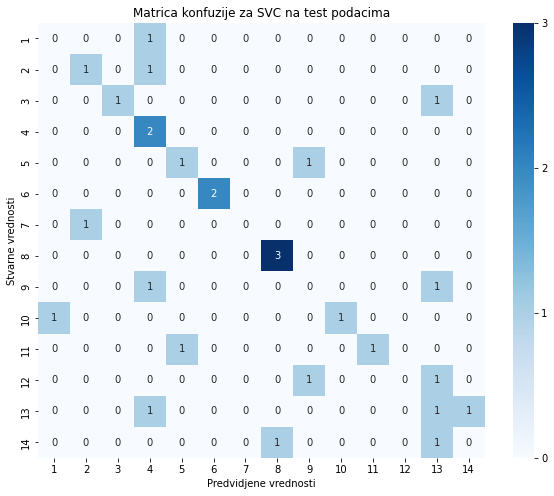
\includegraphics[width=\linewidth]{SVCconf.png}
        \captionsetup{justification=centering}
        \caption*{\textbf{Matrica konfuzije za SVC \\ model.}}
        \label{fig:nedostajuce}
    \end{minipage}%
    \begin{minipage}{0.5\textwidth}
        \textbf{Analiza:}\\
        
        \vspace{1mm}
        Element na poziciji (2, 2): 1\\
        Element na poziciji (3, 3): 1\\
        Element na poziciji (4, 4): 2\\
        Element na poziciji (5, 5): 1\\
        Element na poziciji (6, 6): 2\\
        Element na poziciji (8, 8): 3\\
        Element na poziciji (10, 10): 1\\
        Element na poziciji (11, 11): 1\\
        Element na poziciji (13, 13): 1\\

    \end{minipage}
\end{figure}

Klase 2, 3, 4, 5, 6, 8, 10, 11 i 13 su dobro klasifikovane. Model je tačno klasifikovao po dve instance za klase 4 i 6, a 3 instance za klasu 8. Pored toga u ovoj matrici konfuzije ima najviše nenula elemenata na dijagonali, što ukazuje na to da je SVC model najbolje klasifikovao,  posmatrajući matrice konfuzije.
\end{flushleft}

\newpage



\begin{figure}[ht]
    \centering
    \begin{minipage}{0.5\textwidth}
        \centering
        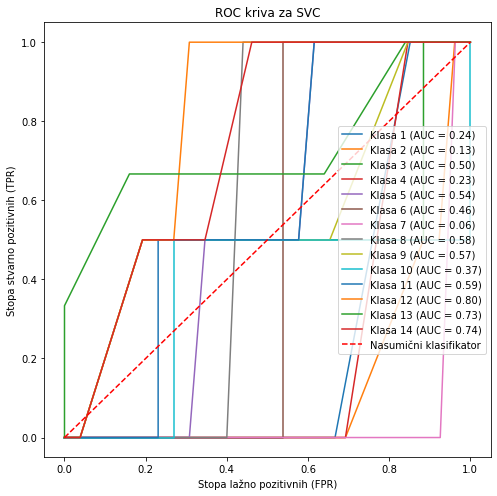
\includegraphics[width=\textwidth]{svcROC.png}
        \renewcommand{\thefigure}{} 
        \captionsetup{labelformat=empty}
        \subcaption{\textbf{ROC krive svih klasa.}}
        \label{fig:udeo1}
    \end{minipage}\hfill
    \begin{minipage}{0.5\textwidth}
        \centering
        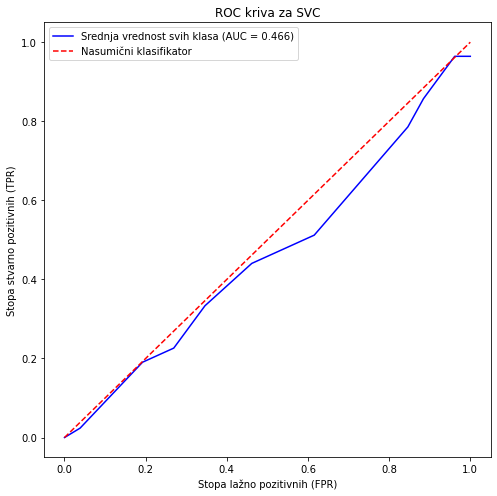
\includegraphics[width=\textwidth]{prosecniROC/svc.png}
        \renewcommand{\thefigure}{} 
        \captionsetup{labelformat=empty}
        \subcaption{\textbf{ROC kriva - prosek svih klasa.}}
        \label{fig:udeo2}
    \end{minipage}
\end{figure}
\begin{flushleft}

Možemo videti da je klasa 12 najbolje klasifikovana, a klasa 7 najgore. Slika b pokazuje ROC krivu proseka svih klasa na kojoj možemo videti da je klasifikator nasumičnog klasifikatora koji prikazuje granicu izmedju lošeg i dobrog klasterovanja uvek iznad naše ROC krive. To znači da je ovaj algoritam ispod proseka u klasifikaciji uzimajući u obzir AUC vrednost i izgled ROC krive.
\end{flushleft}


\newpage


\subsubsection{Uporedjivanje svih modela klasifikacije}

\begin{flushleft}
    \textbf{Support Vector Classifier (SVC): \\
}
Preciznost, odziv i F1-ocena variraju u zavisnosti od klase, ali u globalu nisu izuzetno visoki. Može se primetiti da model nije dobro generalizovan na sve klase, a posebno ima problema sa manje zastupljenim klasama. Model se pokazao najbolje posmatrajući rezultate matrica konfuzije. 

\vspace{2.75mm}
\textbf{Gradient Boosting:}\\

Tačnost i F1 Score su i dalje niski. Bolje prepoznaje neke klase u odnosu na SVC, ali generalno model nije visoko precizan.
\vspace{2.75mm}

\textbf{Random Forest:}\\
Ovaj model takođe pokazuje izazove u efikasnoj klasifikaciji. Postoje problemi u identifikaciji većine klasa.
\vspace{2.75mm}

\textbf{Multinomial Bayes:} \\
Ovaj model se čini manje efikasnim u poređenju sa prethodnim algoritmima. Nizak F1 Score i preciznost ukazuju na to da model nije dobro prilagođen podacima.

\vspace{2.75mm}

Na osnovu svih metrika, SVC se čini kao najbolji model, iako nijedan od modela ne pokazuje izuzetne performanse.

\vspace{2.75mm}

Na sledećoj slici možemo videti odnos tačnosti svih modela.

\vspace{6.75mm}
\end{flushleft}


\begin{figure}[ht]
    \centering
    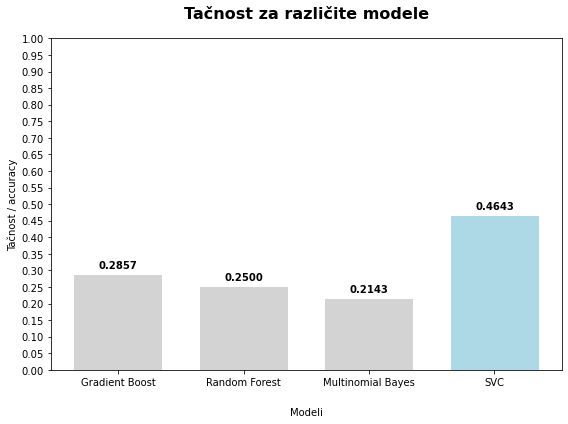
\includegraphics[width=0.6\textwidth]{modeliACC.png}
    \captionsetup{labelformat=empty}
    %\caption*{\textbf{Tačnost za različite modele.}}
    \label{fig:nedostajuce}
\end{figure}
\vspace{2.75mm}

\begin{flushleft}
\textbf{Analiza:}\\

Možemo videti, u poređenju sa ostalim modelima, kao što je već i rečeno, da je SVC najbolji model.
\end{flushleft}


\newpage
\begin{flushleft}

Na sledećoj slici možemo videti ROC krive i AUC vrednosti za iskorišćene modele.
\end{flushleft}

\begin{figure}[ht]
    \centering
    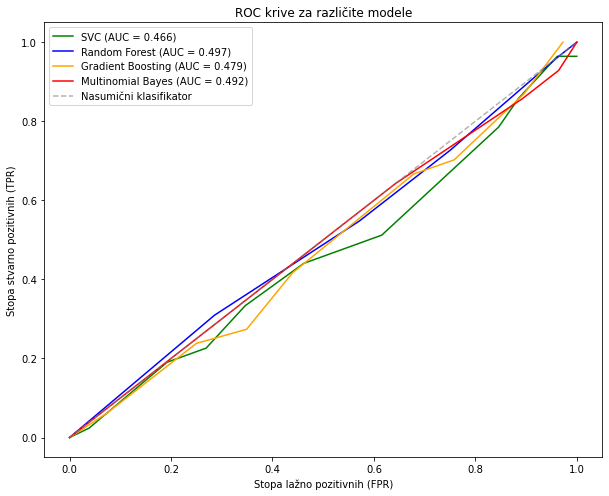
\includegraphics[width=0.6\textwidth]{modeliROC.png}
    \captionsetup{labelformat=empty}
    \caption{\textbf{ROC krive za različite modele.}}
    \label{fig:nedostajuce}
\end{figure}

\begin{flushleft}
\textbf{Analiza:}\\
\vspace{1mm}
    AUC vrednosti su relativno niske, što sugeriše da modeli imaju ograničenu sposobnost razlikovanja klasa. Idealna vrednost za AUC je 1, što znači potpunu razliku između klasa, dok vrednost 0.5 sugeriše na slučajno predviđanje. Tačnost nije visoka ni za jedan od modela. Ovo može ukazivati na to da su modeli generalno manje sposobni da dobro klasifikuju podatke.\\ \vspace{3mm}
Random Forest ima najvišu AUC vrednost, ali i najnižu tačnost, što ukazuje na to da može biti bolji u razlikovanju klasa, ali ne nužno i u ispravnom predviđanju klasa.\\
\vspace{3mm}
SVC ima slične AUC i tačnost vrednosti, što sugeriše na nešto bolje opšte performanse u poređenju s drugim modelima. Što se tiče ROC krive i AUC vrednosti, to je malo lošije od ostalih modela, ali AUC meri ukupnu sposobnost modela da razlikuje između klasa, dok matrica konfuzije pruža detalje o specifičnosti (tačnost negativnih instanci) i osetljivosti (tačnost pozitivnih instanci). Model može biti najbolji u identifikaciji određenih klasa, ali AUC, gledajući celokupnu performansu, može biti niža.\\
\vspace{3mm}
Multinomijalni Bajes ima srednje rezultate, ali bolje od Random Foresta i Gradient Boosting-a.\\
\vspace{3mm}
Gradient Boosting ima najvišu tačnost, ali najnižu AUC vrednost, što ukazuje na to da može biti sklon preprilagođavanju.\\

\end{flushleft}




\newpage



\subsection{SPMF algoritmi}

\subsubsection{Naivni Bajes}
\begin{flushleft}

Algoritam je klasifikator tekstualnih dokumenata implementiran od strane Sabarish Raghu 2015. godine. Može automatski klasifikovati tekstove u kategorije. Na primer, može se koristiti za klasifikaciju teksta po temama. Ulaz su skup tekstova učenja klasifikovanih po kategorijama (sa poznatim kategorijama) i skup tekstova koji treba klasifikovati (sa nepoznatim kategorijama). Izlaz je dodeljivanje kategorije svakom tekstu iz skupa testiranja. \\
\vspace{2mm}

Kako algoritam funkcioniše?\\
Naivni Bajesov klasifikator je probabilistički klasifikator. Računa verovatnoću da dokument \( d \) pripada klasi \( c \) na sledeći način:

\[
P(c|d) \propto P(c) \prod_{1 \leq k \leq n_d} P(t_k | c)
\]

gde je:
\begin{align*}
& n_d \text{ - dužina dokumenta (broj tokena)}, \\
& P(t_k | c) \text{ - uslovna verovatnoća da se pojam } t_k \text{ javlja u dokumentu klase } c, \\
& P(t_k | c) \text{ - merilo koliko dokazi } t_k \text{ doprinose tome da je } c \text{ ispravna klasa}, \\
& P(c) \text{ - apriori verovatnoća klase } c, \\
& \propto \text{ - oznaka za proporcionalnost}.
\end{align*}

Ako pojmovi dokumenta ne pružaju jasne dokaze za jednu klasu u odnosu na drugu, biramo klasu sa najvišom \( P(c) \).


\vspace{4mm}

Podela na trening i test skupove je izvršena na samom kraju spmf.ipynb datoteke. Napravljeni su direktorijumi pod nazivom \verb|"Testiranje"| i \verb|"Trening"|. U direktorijumu \verb|"Testiranje"| se nalaze fajlovi sa tekstovima, a u direktorijumu \verb|"Trening"| se nalaze zasebni folderi za svakog autora. 
Sve dalje je samo izmena postojećeg koda, preuzetog sa sajta, koji se može pronaći u referencama. U Main.java datoteci, su postavljeni navedeni direktorijumi za odgovarajuće, a za izlazni direktorijum je podešen direktorijum Izlaz u kom se, posle pokretanja, generiše output.tsv datoteka.
\vspace{2mm}

Rezultati ovog algritma su veoma loši. Testiranjem ovog algoritma više puta, on dobro klasifikuje samo klase koje u tom momentu imaju najviše podataka u Treningu.

\end{flushleft}

%\newpage
\vspace{2.5mm}


\subsubsection{Klasterovanje}
\begin{flushleft}


Algoritam je implementiran od strane Sabarish Raghu- a 2015. godine. Može automatski grupisati tekstove u klasterima. Osim toga, pruža mogućnost izvođenja, korenčanja i uklanjanja zaustavnih reči pre nego što izvrši klasterovanje.\\

\vspace{3mm}
Klasterovanje teksta se odvija na sledeći način:\\

1. Učitaj ulazni fajl.\\
2. Ukloni zaustavne reči (opciono).\\
3. Pronađi koren reči (opciono).\\
4. Izračunaj vrednost tf*idf za svaki zapis u ulaznom fajlu.\\
5. Izračunaj matricu sličnosti koristeći vrednosti tfidf zapisa.\\
6. Odaberi najsvrsishodnije zapise za svaki zapis i prvobitno ih formiraj u klasterima.\\
7. Koristi pravilo tranzitivnosti: A, B su najsličniji, zatim B, C su najsličniji; to ukazuje da su A i C verovatno slični. Ovo implicira da su A, B, C u istom klasteru.\\
8. Spoji klaster na osnovu navedenog pravila za sve zapise.\\
9. Zapiši konačni izlaz, odnosno konačne skupove klastera u izlazni fajl.\\

\vspace{3mm}

Program koji vrši naredne operacije se nalazi u spmf.ipynb datoteci.
\vspace{3mm}
\newpage
Uvozi se biblioteka spmf. Iskorišćen je medjukorak iz classla programa tj. rađeno je nad classla\textunderscore medjukorak.csv datotekom na početku, gde su sve promene u bazi sačuvane u sorted\textunderscore file.txt datoteci. Promene koje su izvršene su sortiranje prema autoru i pravljenje nove kolone \verb|"Tekst"|, koja nastaje pretvaranjem vrednosti iz kolone \verb|"Procesiran tekst"|u liste, a kasnije se kolone \verb|"Autor"| i \verb|"Procesiran tekst"| brišu iz baze.
Poziva se SPMF biblioteka sa odgovarajućim argumentima. Odgovarajući algoritam je \verb|"TextClusterer"|, a fajl na kom se radi je naš sorted\textunderscore file.txt. Izlazni fajl je clusters.txt. Iz biblioteke matplotlib uvozimo klasu ListedColormap, radi vizuelizacije rezultata klasterovanja. Na sledećoj slici možemo videti rezultate.

\begin{figure}[ht]
    \centering
    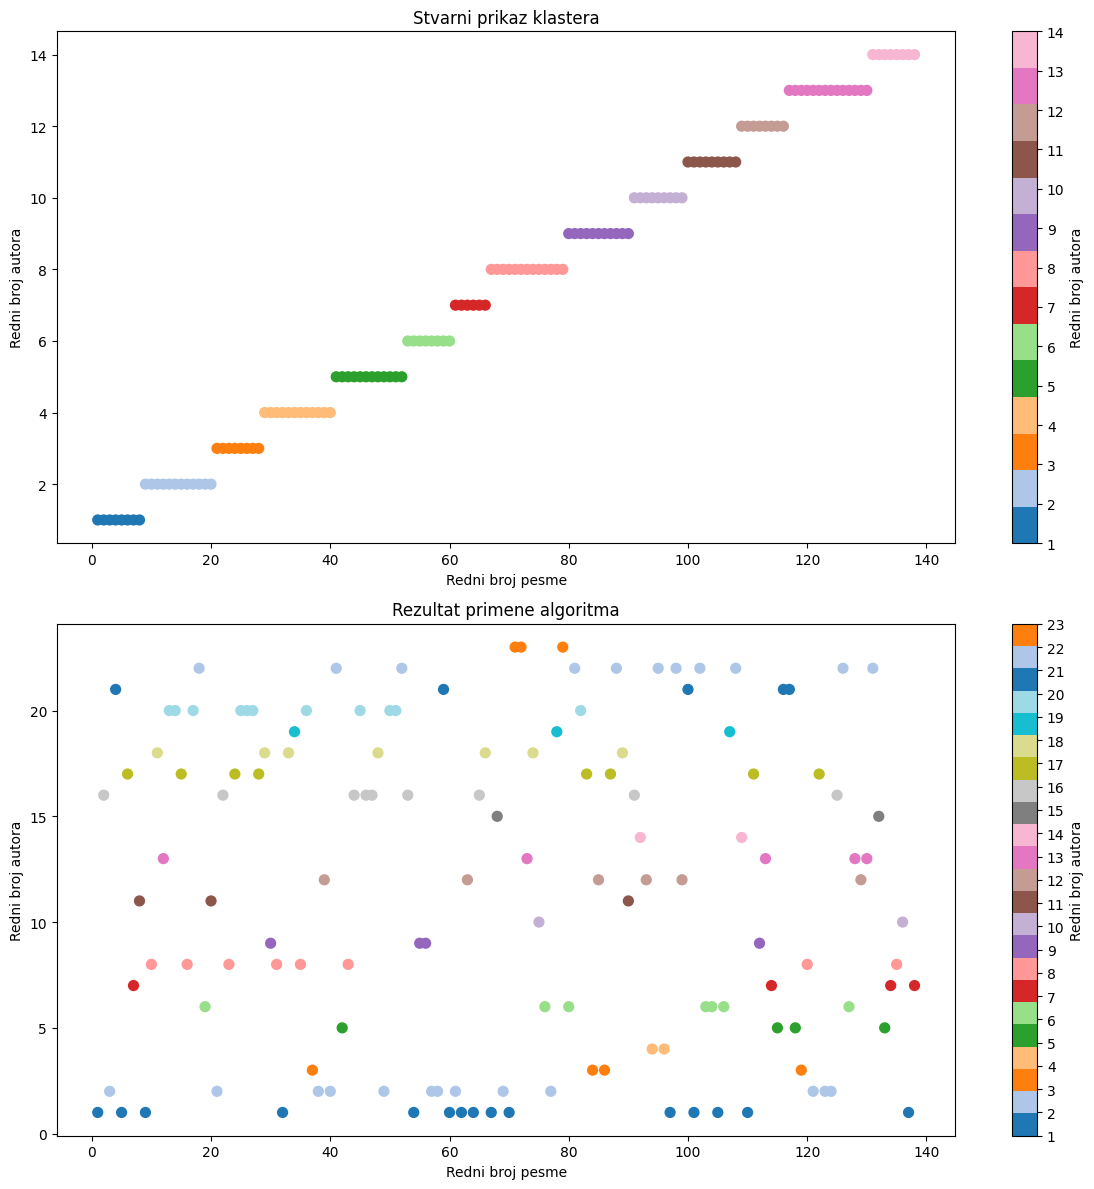
\includegraphics[width=0.6\textwidth]{klasterovanje.png}
    \captionsetup{labelformat=empty}
    \caption{\textbf{Rezultati klasterovanja.}}
    \label{fig:nedostajuce}
\end{figure}

\textbf{Tačnost ovog algoritma:} 0.014 \\
\vspace{3mm}

Rezultati nisu zadovoljavajući. Najgori tip klasterovanja je onaj kada je svaka klasa zaseban klaster. To znači da algoritam nije uspeo ni na koji način da spoji više klasa po nekoj osobini u odgovarajući klaster. Na ovoj slici se može videti takav slučaj, što pokazuje na loše performanse algoritma. Takođe, tačnost samog algoritma je jako loša.
\end{flushleft}




\newpage

\section{Zaključak}

\begin{flushleft}


Rad s malom bazom podataka predstavlja izazov u izradi efikasnog modela koji 
precizno predviđa rezultate, a dodatni problem predstavlja još manji korpus reči 
nakon podele na trening i test skupove. Ova situacija ograničava kapacitet modela 
da se efikasno prilagodi nepoznatim podacima.\\

\vspace{10pt}

U cilju prevazilaženja ovih izazova, odlučili smo se za korišćenje raznih 
biblioteka, analiza i modela gde se Classla biblioteka najbolje pokazala, pri čemu
smo ostvarili najbolje rezultate primenom Support Vector Classification (SVC) 
modela na podacima obrađenim kroz niz funkcionalnosti koje ova bliblioteka pruža. \\
\vspace{10pt}

Stil pisanja predstavlja jako interesantan aspekt analize, s obzirom na brojne 
faktore koji utiču na prepoznavanje određenog autora. Projekat je postao izuzetno 
zanimljiv zbog ove kompleksnosti, istovremeno pružajući izazov u razumevanju 
varijacija u stilu pisanja.\\

\vspace{10pt}

Uprkos svim izazovima, ovaj projekat nije samo pružio dublje razumevanje značaja 
stila, već je takođe istakao važnost pravilnog pristupa pri radu s ograničenim 
resursima, pri čemu smo dosta novog naučili.


\end{flushleft}
\newpage



\section{Reference}

\begin{flushleft}
\texttt{[1]}  \href{https://huggingface.co/docs/datasets/index}{Biblioteka 
datasets}\\
\texttt{[2]}  \href{https://www.tensorflow.org/overview}{Biblioteka tensorflow} \\
\texttt{[3]}  \href{https://scikit-learn.org/stable/}{Biblioteka sklearn} \\
\texttt{[4]}  \href{https://pypi.org/project/classla/}{Biblioteka Classla}  \\
\texttt{[5]}  \href{https://github.com/huggingface/setfit}{Biblioteka Set-fit}\\
\texttt{[6]}  \href{https://pandas.pydata.org/docs/reference/index.html#api}
{Biblioteka pandas } \\
\texttt{[7]}   \href{https://www.nltk.org/}{Biblioteka za obradu jezika nltk}\\
\texttt{[8]} \href{https://www.sbert.net/}{Biblioteka Sentence Transformers} \\
\texttt{[9]} \href{https://docs.python.org/3/howto/regex.html}{Ugrađeni modul u 
standardnoj Python biblioteci za rad sa regularnim izrazima - re} \\
\texttt{[10]}  \href{https://huggingface.co/sentence-transformers/paraphrase-multilingual-mpnet-base-v2}{Model sentence-transformers/paraphrase-multilingual-mpnet-base-v2} \\
\texttt{[11]}  \href{https://www.poezijanoci.com/domaca-poezija.html}{Sajt sa kog 
su preuzeti dodatni tekstovi pesama - "Poezija noći"} \\
\texttt{[12]} \href{https://www.philippe-fournier-viger.com/spmf/index.php?link=algorithms.php}{SPMF biblioteka}\\
\texttt{[13]} \href{https://matplotlib.org/stable/api/index}{Biblioteka matplotlib}\\
\end{flushleft}



\end{document}